\chapter{Calibration} \label{chap:cal}

Calibration is a common component of any precision system for good reason. For this project it will be used to check if the scanner system is capable of accurately replicating the intended geometry and if not, adjust it so that it does. In section \ref{sec:f-theta-model} it is described how the f-theta in principle establishes a linear relation between the mirror angles and the position of the melt pool. One purpose for calibration is to determine the coefficients of this linear relation. However, as seen in Section \ref{sec:f-theta-dev}, the f-theta lens is not entirely capable of enforcing a linear relation, so the purpose of the calibration can be extended to help better establish the linear relation.

The system in need of calibration has to be defined by a mathematical model. In our case that system is the whole process, as described in the introduction, from inputting the desired (nominal) coordinates for a point on print all the way to the position of that point on the finished print. That whole process can be modelled as a function $f: (x_{nom}, y_{nom}) \rightarrow  (x_{meas}, y_{meas})$ with \textit{nom} short for nominal and \textit{meas} short for measured. The calibration works by deriving a function $f^{-1}: (x_{meas}, y_{meas}) \rightarrow  (x_{nom}, y_{nom})$ such that $f(f^{-1}): x, y \rightarrow  x, y$ (is the identity function). In other words: A function $f^{-1}$ such that if the desired geometry is parsed through $f^{-1}$ before inserting it into the print process the output will be that desired geometry. 

It is tempting to do this by generating a data set of $(x_{nom}, y_{nom}, x_{meas}, y_{meas})$ points and fit a function $g_{fit}: (x_{meas}, y_{meas}) \rightarrow  (x_{nom}, y_{nom})$, but this is not strictly the same as the above mentioned $f^{-1}$. The fitted function $g_{fit}$ might be fit for purpose, and under some conditions it might even be identical to $f^{-1}$. However without a deep dive into the workings of the statistical methods behind the fit, it cannot be guaranteed, so instead a slightly more elaborate approach has been pursued. A function $f_{fit}: (x_{nom}, y_{nom}) \rightarrow  (x_{meas}, y_{meas})$ must first be fitted to the data, which gives expressions for $x_{meas}$ and $y_{meas}$ as functions of $x_{nom}$ and $y_{nom}$. Then these two expressions are solved for $x_{nom}$ and $y_{nom}$ as functions of $x_{meas}$ and $y_{meas}$. Thus, by providing the desired position to the these function it is possible to calculate the required input to actually make the laser hit the desired location within the image plane. That is the desired $f^{-1}$.

After $f^{-1}$ is known, there also needs to be a way to implement the result back in the system and to evaluate if the performance has improved and is satisfactory.

The whole process consists of the following steps:
\begin{enumerate}
    \item Produce calibration medium (CAD file, g-code, manufacture print)
    \item Measure calibration medium (automation of measurements, proper procedure)
    \item Analyse measurements (regression, prepare for implementation)
    \item Reimplement results (g-code parser)
    \item Produce control medium (CAD file, g-code, manufacture print)
    \item Measure control medium (automation of measurements, proper procedure)
    \item Analyse measurements (check if accuracy has improved)
    \item Succes or rejection
\end{enumerate}

In the following sections it is described how methods have been chosen and developed for each of the steps, how the calibration has been done and the procedure used to check if it worked. A diagram to illustrate the calibration system is presented on Figure \ref{fig:calibration-system}.

\begin{figure}
    \centering
    \includesvg[width=\linewidth]{Pictures/calibration-system-font-to-path.svg}
    \caption{An overview of the system used to calibrate the scanner movement in a L-PBF system. The red arrows indicate the calibration process and the blue arrows the verification process.}
    \label{fig:calibration-system}
\end{figure}

\section{Calibration medium design}

A design is needed that can be produced, measured and analysed, to show the relevant characteristics of the L-PBF system with sufficient precision.

A grid pattern of dots is good for this purpose, because it gives data about a wide range of (x,y)-positions of the melt pool and covers the whole scan field, which is square. Instead of printing actual 3d-structures, markings are made on a metal plate with the laser. A single point with the laser is hard to detect/define, so each of the dots is printed as a circle. By detecting the perimeter of the circle, the centre can be determined with robust precision. Even if the edge of the circle is a bit ragged or hard to define, the centre is precise, because the uncertainties are evenly distributed around the centre.

The scan field of the Baxter is square with 125mm on each side. To match this, a design with 11 times 11 circles of 5mm diameter and 10mm centre-to-centre distance was created. The first iteration had only 9x9 circles but it was extended to better quantify errors that are present farther from the centre and to provide more data to work with in the data analysis. 

For larger scan fields it is sensible to increase the spacing of the grid, so that the pattern reaches the edge of the scan field, where distortions generally become more apparent \cite[Figure 2.35]{sebastian-phd}.

These specifications for the grid pattern were combined to a CAD-file by Sebastian Aagaard Andersen which is uploaded as an attachment file at Appendix \ref{app:repository}

The pattern was printed on a sturdy plate. It was discovered that if the plate gets bent a little it becomes very hard to get a consistent focus during the optical measurements. Also, the plate should have high contrast between marked and unmarked areas. The matte black anodised aluminium worked well because the anodised layer was removed by the laser markings. The measurement process is explained in depth in Section \ref{sec:cal-meas}.

\section{Calibration medium production} \label{sec:cal-medium-prod}

The L-PBF system is designed to produce 3D structures, by consolidating a powdered metal feedstock layer by layer into a solid geometry. In contrast the markings for the calibration are flat and made without metal powder. To work around this difference, the "layer height" was set so that the L-PBF system marked the same circles multiple times with different line angles, giving a more even and clean hatching.

The complete settings for the calibration medium production are listed in Table \ref{tab:scan-settings}.

\begin{table}[h]
\centering
    \begin{tabular}{l|l}
        \textbf{Setting} & \textbf{Value} \\ \hline
        Hatching strategy & parallel lines \\
        Hatching density & 100\% \\
        Hatching overlap & 0\% \\
        Hatching rotation & 67$^\circ$ \\
        Hatching laser power & 30 W \\
        Hatching scan speed & 200 mm/s \\
        Hatching duty cycle & 100\% \\
        Hatching frequency & 100 kHz \\
        Building area width & 125 mm \\
        Layer thickness & 1000 $\mu$m\\
        Laser width & 80 $\mu$m\\
        Laser-off scan speed & 2000 mm/s
    \end{tabular}
    \caption{Scan settings}
    \label{tab:scan-settings}
\end{table}

A low scan speed was decided because the experiment is about the static properties of the printer, so the influence high speeds might have on the scan paths should be avoided. The low scan speed was combined with low laser power, which was needed because high laser power causes rapid thermal expansion of the print plate. 20W showed not to be enough to make any markings at all. 30W worked but already caused sparks which made very unfortunate markings on the plate that disturbed the automated optical measurements. More on this in Sectin \ref{sec:filtering}.

The distance between the hatching was set to be small because ideally the marked surface should be uniform and not show scan lines at all. Even with the laser width of 80 $\mu m$ there were black lines between the paths, so even tighter lines would probably be reasonable.
Also 67$^\circ$ rotation between layers was used because this is standard and gives a good variation in scan angles for five layers avoiding that the directions of the scan paths become colinear with one of the previous layers.

With these settings the g-code that specified the commands for the printer was produced. The powder recoatings were removed completely from the g-code, because no powder was used as mentioned earlier. The contours were removed as well, because the movement algorithm used in the Baxter at the time caused some print-irregularities on the perimeter. Besides these exception the calibration medium production was carried out as close to normal production conditions as possible. The mirrors were cooled and the build chamber flushed with nitrogen.

For the optical measurements to work it was also important to make sure that the calibration medium didn't get any scratches during the transport from the production machine to the measurement machine.

\section{Calibration measurements}\label{sec:cal-meas}

The goal of the measurements was to get as accurate a measurement of the circle centres as possible. The calibration medium (deliberately) had many measurement points and a high precision was desired, which motivated the choice for an automated measurement instrument, namely the DeMeet 220 with Approve for DeMeet v3.4.

The calibration print was fixated in the DeMeet by a flat ground plane, two stops on one edge, another stop on a second edge and some sticky tack to stop the plate from sliding during measurements.

The automated optical circle measurement feature of the DeMeet worked by surveying a doughnut shaped field with the centre in the expected centre of the circle as shown on Figure \ref{fig:doughnut}. The centre of the search was set to the nominal position of the centre, and the width of the doughnut was set such that there was a 1 mm margin both inside and outside the circle perimeter, where the DeMeet would try to identify the perimeter. The same inward and outward error margin is used because any deviation from the nominal circle is expected to come from a wrong centre, while the diameter is assumed to be more or less correct. This means, that whatever is the smallest error margin will be transgressed first so nothing is won by making one larger than the other (/smallest).

\begin{figure}
    \centering
    \includesvg[width=0.5\linewidth]{Pictures/donut-search-field.svg}
    \caption{An illustration of how the search field for the automated detection was chosen to ensure that the circles would be detected even if the centres were displaced or the diameter was incorrect. The transparent blue doughnut-shaped area is the search field and the light grey circle (partly overlapping with the search field) is the actual printed circle. In this example the perimeter of the actual circle is entirely inside the search field and would thus be detected correctly}
    \label{fig:doughnut}
\end{figure}

The circle perimeter search worked by edge-detection, and the standard approach to determine the circle perimeter was to do a best-$R^2$-fit. This didn't work for these calibration measurements though because the edge-detection would wrongly identify brightness changes in the circle fill as the actual edge on the perimeter. What worked instead was to use a minimum-circumscribed fit, since only very few erroneous edges were detected outside the circle perimeter.

The whole calibration is mostly aimed at correcting relative errors. That is, the distances from the centre to other points of the print. The absolute placement of the centre on the build plate and also rotation around the centre are less important since the print will be cut away from the build plate in the end anyway. Because of this no attention was paid to fixate the plate in an identical way in the printer and DeMeet. Instead a procedure was devised to align a coordinate system in the DeMeet, based on points of the print that could be assumed to have no distortion.

\begin{figure}
    \centering
    \includesvg[width=\linewidth]{Pictures/calibration-grid.svg}
    \caption{The grid of circles used in the calibration. The coordinate systems of the L-PBF system Baxter and measurement instrument DeMeet are shown together with the anchor points used to align the coordinate system of the DeMeet. The red points are used to rotate the x-axis and the green points are used to locate the origo.}
    \label{fig:calibration-grid}
\end{figure}

This alignment procedure is illustrated in Figure \ref{fig:calibration-grid} and was designed to put origo on the centre circle, since this is where the error from the printer could be expected to be the smallest. The printer uses a left hand coordinate system, while the DeMeet uses a right hand coordinate system, so it was chosen to have the x-axis point in the same direction and y-axis in opposite directions. This is taken into account when processing the data in Section \ref{sec:cal-cal}. Each step of the alignment procedure starts by manually placing a marker that is tangent to one of the circles and based on this, the alignment script will then adjust the coordinate system automatically. The full procedure is specified here:

\begin{enumerate}
    \item Start with the default coordinate system of the DeMeet
    \item Find the top tangent point of the (0,0)-circle and let this be the preliminary origo
    \item Find the top tangent point of the (50,0)-circle and rotate the x-axis to go through this point
    \item Find the right tangent point of the (0,0)-circle, the right tangent point of the (50,0) circle, and the top tangent of the (0,50)-circle and use these three points to shift define the x- and y-axis into position
\end{enumerate}

The trickiest part of the measurements was getting the edge-detection right. First off, the surface needed to be cleaned with lens wipes and compressed air. Once in the measurement apparatus, the correct focus needed to be found. For this it was important to have a flat plate. A bend plate made it impossible to be in focus for all measurement points. Lastly, the right amount of lighting was important. Too little light and the edge-detection wouldn't pick up sufficiently a sufficient amount of points on the perimeter to get a clear picture of the full circle. Too much light, and the edge-detection would pick up spots outside of the circle as if they were part of the circle. The more scratches and dust there was on the plate, the higher the chance of that kind of error. What seemed to be the biggest problem though was marks that were caused presumably by sparks that had landed on the build plate. These caused errors that could not be avoided and needed to be filtered out in the data analysis (see Section \ref{sec:cal-cal}).

\begin{figure}[ht]
    \centering
    \begin{subfigure}{0.32\textwidth}
        \centering
        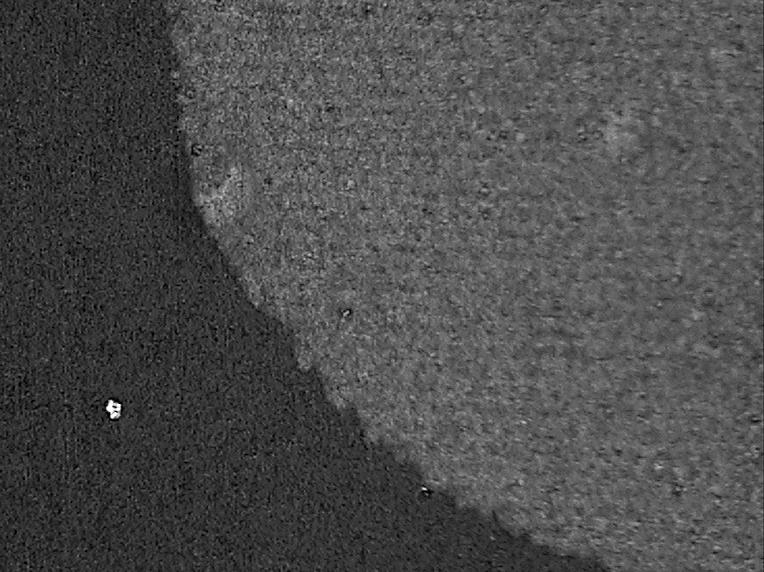
\includegraphics[width=\linewidth]{Pictures/spark-mark.jpeg}
        \caption{A mark outside the circle, probably caused by a spark landing back on the plate}
        \label{fig:spark-mark}
    \end{subfigure}
    \begin{subfigure}{0.32\textwidth}
        \centering
        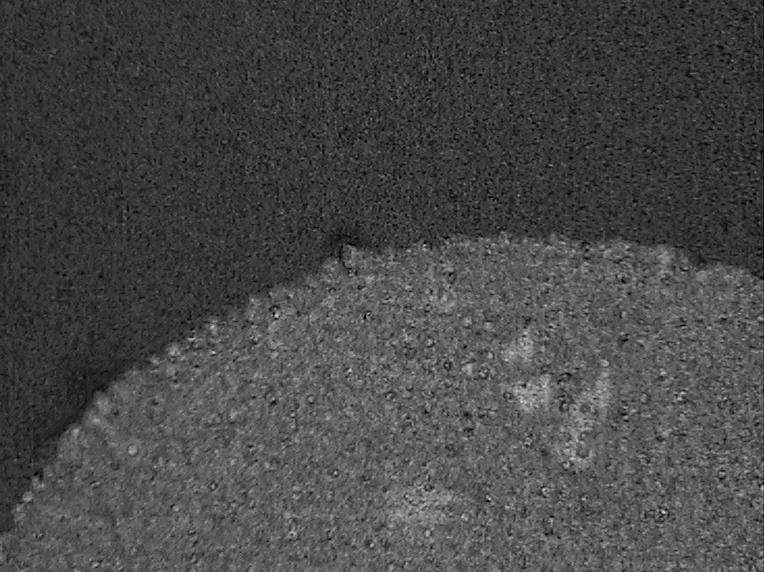
\includegraphics[width=\linewidth]{Pictures/bump.jpeg}
        \caption{A bump at the perimeter}
        \label{fig:bump}
    \end{subfigure}
    \begin{subfigure}{0.32\textwidth}
        \centering
        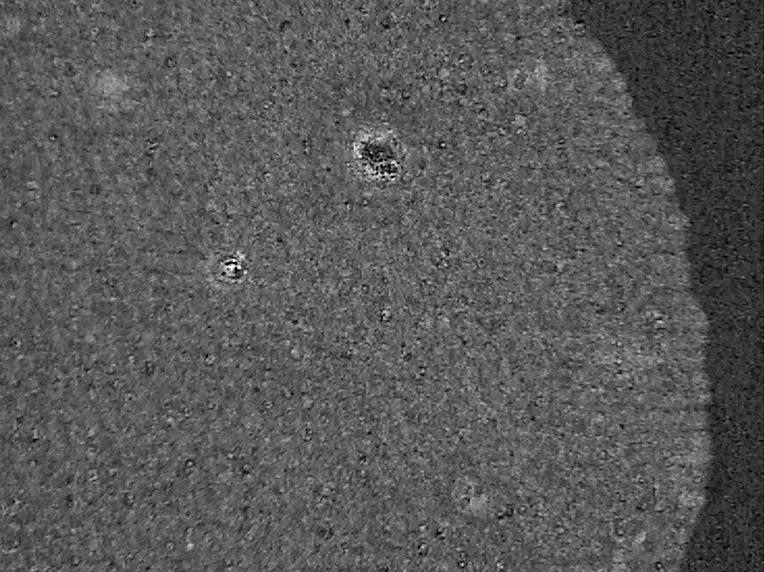
\includegraphics[width=\linewidth]{Pictures/crater.jpeg}
        \caption{A "crater" - this print error doesn't influence the measurement accuracy by itself, but could be origin to the sparks}
        \label{fig:crater}
    \end{subfigure}
    \caption{Different sources of errors for the automated circle detection}
    \label{fig:meas-error-sources}
\end{figure}

The data collected for each of the 121 circles are the following:
\begin{itemize}
    \item The measured (x,y)-coordinates of the centre
    \item The nominal (x,y)-coordinates of the centre
    \item The measured diameter
    \item The nominal diameter
\end{itemize}
The full measurement data can be reviewed in Appendix \ref{app:calibration-data}.

\section{Calibration correction calculations} \label{sec:cal-cal}
Having obtained the measurements, the next step is to analyse them to find systematic errors. This data processing takes three steps, each of which needs some consideration to design. A way to assess the quality of the measurements must be developed to filter outliers. Then an appropriate expression to fit the data to must be determined. Lastly it must be derived from the results of the fit how the nominal values should be adjusted.

\subsection{Filtering outliers} \label{sec:filtering}
The need to filter the raw measurement data comes from the fact that unfortunately some of the data points don't represent the centre of the actual circles on the print very well. So, to be clear, this section is not about the fact that the centres of the actual circles are off from the nominal position they are supposed to be at. Instead, the filtering is about that the measured values of the centres of a few of the circles are not the same as the actual centres of those circles. As mentioned earlier, this relates to the spark marks that were erroneously included in the detected "circle". These cases are identified by their excessive diameter and can be filtered out based on that, see Figure \ref{fig:cal-out-diam}. As can be seen on Figure \ref{fig:cal-out-pos}, the resulting filtered points are randomly distributed across the scan field. Also the filtering is based on diameter while it's the positions that are used in the data analysis so the filtering will thus not result in a bias of the analysis.

\begin{figure}
\centering
\begin{subfigure}{0.72\textwidth}
  \centering
  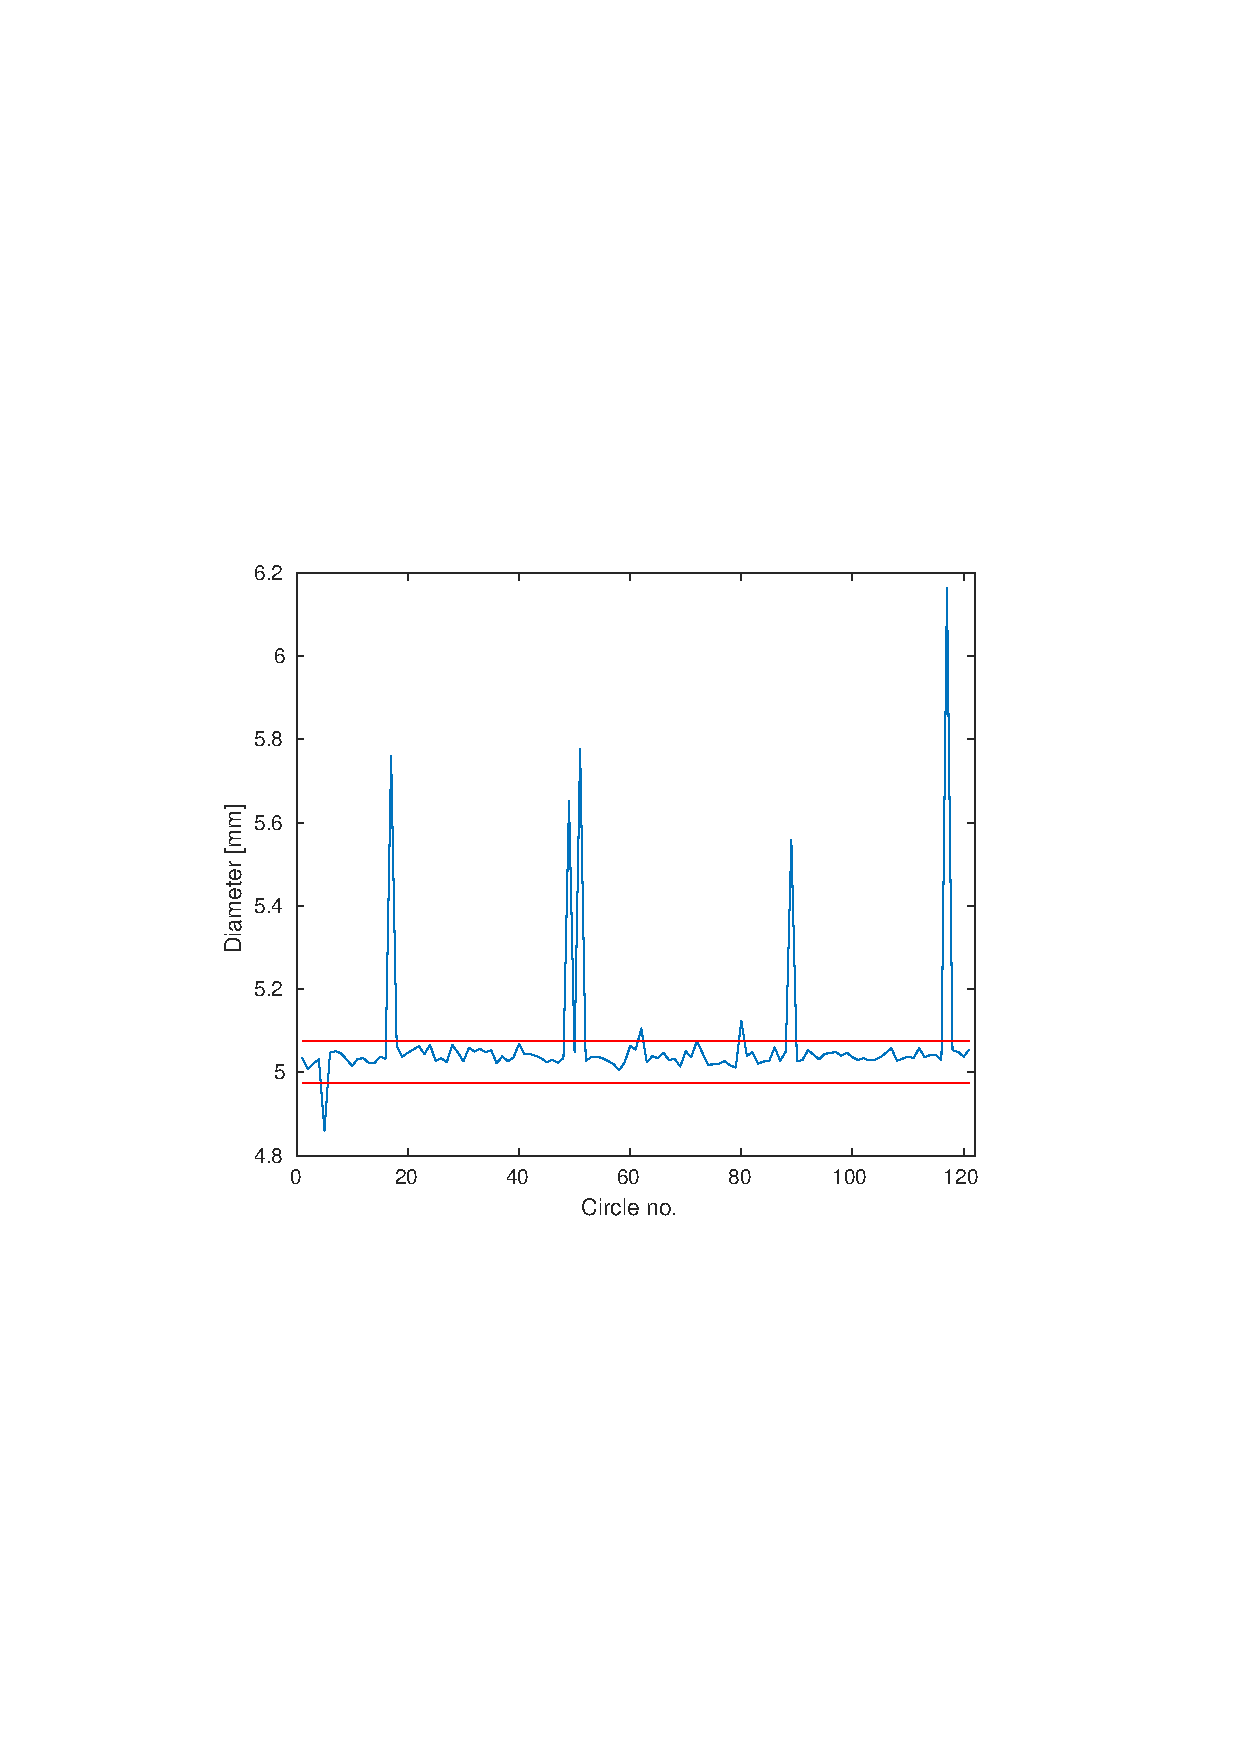
\includegraphics[clip, trim=3.5cm 8cm 3.5cm 8cm, width=\linewidth]{Pictures/cal-outliers-diameter.pdf}
  \caption{The diameters of all the detected circles and the lines showing what is considered outliers}
  \label{fig:cal-out-diam}
\end{subfigure}
\begin{subfigure}{0.72\textwidth}
  \centering
  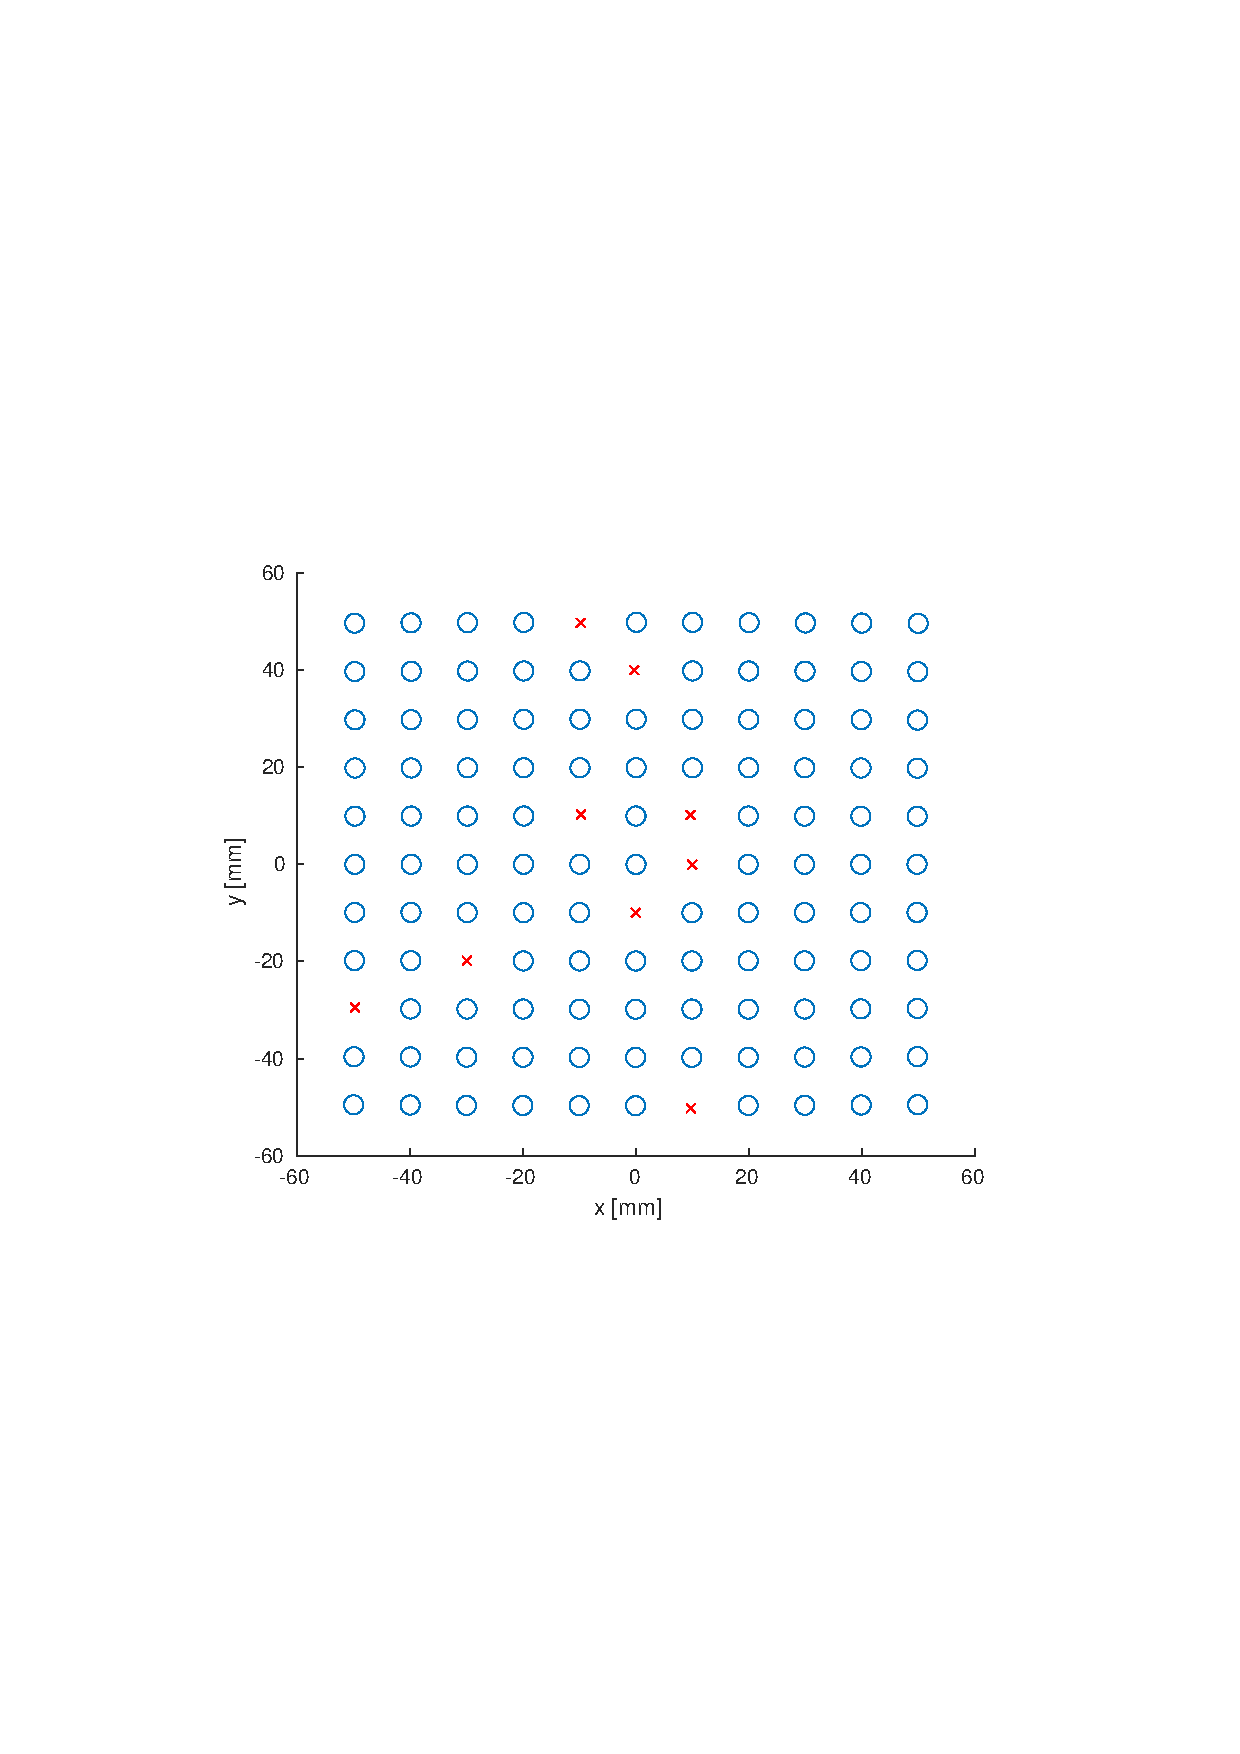
\includegraphics[clip, trim=3.5cm 8cm 3.5cm 8cm, width=\linewidth]{Pictures/cal-outliers-position.pdf}
  \caption{The positions of the circles and the outliers (marked as crosses)}
  \label{fig:cal-out-pos}
\end{subfigure}
\caption{}
\label{fig:filtering-outliers}
\end{figure}

On figure \ref{fig:cal-out-diam} it can also be seen that the diameters are generally slightly larger than 5 mm. This does not necessarily mean that the printer prints too large in general. Most likely, this is an artefact coming from the width of the scan paths.

\subsection{The fit} \label{sec:the-fit}

With the data measured and filtered, the function $f: (x_{nom}, y_{nom}) \rightarrow  (x_{meas}, y_{meas})$ as mentioned in the beginning of the section can be estimated. This function is two functions really, one for each of the output values. It is assumed that these two functions are of the same form but with different coefficients. This follows from the observation made in Section \ref{sec:f-theta-dev-dist} that the difference in mirror position results in different coefficients for x- and y- directions.

The form of $f$ must be sufficiently general to work for different L-PBF systems, but specific enough to be able to work with (it can't contain too many coefficients). From the study of Taylor polynomials, it is known that any (infinitely differentiable) function can be approximated arbitrarily well by a polynomial \cite[eNote 4]{mat1-efterår}. So even though the "true" behaviour of $f$ is a combination of geometric and optical distortions it is a fruitful and sufficiently general approach to use a polynomial form for $f$ \cite{correction-cals}. Polynomials also have the advantage of being computationally easier than for instance trigonometric functions.

The observation made in Section \ref{sec:f-theta-dev-angle}, that the coordinates are interdependent, means it should be a polynomial function with two free variables, namely $x_{nom}$ and $y_{nom}$. This still leaves a vast range of different options for the form: Polynomials can be of arbitrary high order and each of the lower order terms can be included or left out.

The search can be narrowed down by assuming that $f$ is symmetrical when mirrored in either of the $x_{nom}$-axis or $y_{nom}$-axis. That is, the error on $x_{meas}$ is the same (but with opposite sign) whether measured at $+x_{nom}$ or $-x_{nom}$ and (with the same sign) for $+y_{nom}$ or $-y_{nom}$. This is a reasonable assumption because the effects that are suspected to cause the error (described in Section \ref{sec:f-theta-dev}) have this symmetry. The manual of the f-theta (Reference \cite{f-theta-lens-spec}) lens also shows this symmetry.

With this symmetry observation a lot of terms can be excluded from the search for what type of polynomial is best suited. For instance the term $x_{nom}^2$ becomes obsolete in estimating $x_{meas}$ because any positive correlation measured at some $+x_{meas}$ will be mirrored by a negative correlation at $-x_{meas}$ (because $x_{nom}^2$ is always positive). In that way all contributions to the correlation between $x_{nom}^2$ and $x_{meas}$ will cancel out, and the coefficient will come out as 0.

To determine if a term falls under this symmetry case, the signs of the term in the four different quadrants can be investigated to check if it matches that of the variable it is used to estimate. The term must have the same sign as the variable it is supposed to explain in all four quadrants to avoid the described cancellation-by-symmetry effect and get a meaningful correlation and (See Figure \ref{fig:signs-in-quadrants}).

\begin{figure}[ht]
\centering
\begin{subfigure}{.25\textwidth}
  \centering
  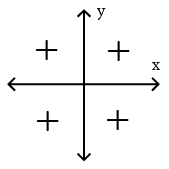
\includegraphics[width=0.9\linewidth]{Pictures/signs-in-quadrants-all-plus-cropped.png}
  \caption{The constant term, 1}
  \label{fig:sign-1}
\end{subfigure}
\begin{subfigure}{.25\textwidth}
  \centering
  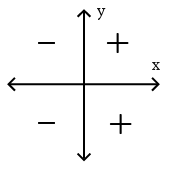
\includegraphics[width=0.9\linewidth]{Pictures/signs-in-quadrants-vertical-cropped.png}
  \caption{The term x}
  \label{fig:sign-x}
\end{subfigure}
\begin{subfigure}{.25\textwidth}
  \centering
  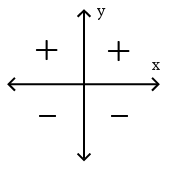
\includegraphics[width=0.9\linewidth]{Pictures/signs-in-quadrants-horisontal-cropped.png}
  \caption{The term y}
  \label{fig:sign-y}
\end{subfigure}
\begin{subfigure}{.25\textwidth}
  \centering
  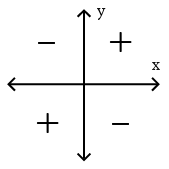
\includegraphics[width=0.9\linewidth]{Pictures/signs-in-quadrants-diagonal-cropped.png}
  \caption{the term xy}
  \label{fig:sign-xy}
\end{subfigure}
\begin{subfigure}{.25\textwidth}
  \centering
  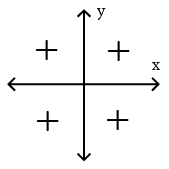
\includegraphics[width=0.9\linewidth]{Pictures/signs-in-quadrants-all-plus-cropped.png}
  \caption{the term $x^2$}
  \label{fig:sign-x2}
\end{subfigure}
\begin{subfigure}{.25\textwidth}
  \centering
  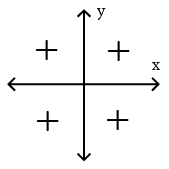
\includegraphics[width=0.9\linewidth]{Pictures/signs-in-quadrants-all-plus-cropped.png}
  \caption{the term $y^2$}
  \label{fig:sign-y2}
\end{subfigure}
\begin{subfigure}{0.25\textwidth}
  \centering
  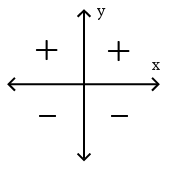
\includegraphics[width=0.9\linewidth]{Pictures/signs-in-quadrants-horisontal-cropped.png}
  \caption{the term $x^2y$}
  \label{fig:sign-x2y}
\end{subfigure}
\begin{subfigure}{.25\textwidth}
  \centering
  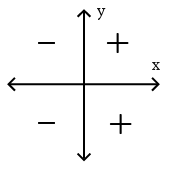
\includegraphics[width=0.9\linewidth]{Pictures/signs-in-quadrants-vertical-cropped.png}
  \caption{the term $xy^2$}
  \label{fig:sign-xy2}
\end{subfigure}
\caption{The signs of the smallest terms of a two-variable polynomial in the four quadrants. It shows that only the terms x and $xy^2$ have the same sign as x, and equally only the terms y and $x^2y$ have the same sign as y}
\label{fig:signs-in-quadrants}
\end{figure}

There are two terms though for which the assumption of symmetry can't be justified. They are the constant term and the term of first order of the "opposite" variable eg. $y_{nom}$ in the expression for $x_{meas}$. Because the coordinate system is aligned semi-manually and thus imperfectly for the measurements, one cannot be sure that the position of the centre and direction of the axis are exactly the same as in the build chamber. These differences mean that it makes sense to include the two terms respectively even though they would be irrelevant based on the earlier symmetry assumption. The most important reason to include the two terms is to avoid that errors caused by shift or rotation of the coordinate system will be counted as something else by the regression.

With above considerations in mind, the test for the simplest models with a satisfying goodness of fit are made. Three different models are fitted to the data and the resulting coefficients of the regression can be seen in Tables \ref{tab:cal-fits-x} and \ref{tab:cal-fits-y}.

\begin{table}[ht]
    \begin{tabular}{l|cccc|c|c}
        $f_x: (x_{nom}, y_{nom}) \rightarrow x_{meas}$ & 
        $q_{x00}$ & $q_{x10}$ & $q_{x01}$ & $q_{x12}$ & $SSE$ \\
        \hline $x_m = q_{x00} + q_{x10}x_n$ & 
        0.0475 & 0.9957 &            &            & 0.3838\\  
        $x_m = q_{x00} + q_{x10}x_n + q_{x01}y_n$ & 
        0.0475 & 0.9958 & 0.0014 &            & 0.1467\\
        $x_m = q_{x00} + q_{x10}x_n + q_{x01}y_n + q_{x12}x_ny_n^2$ & 
        0.0476 & 0.9946 & 0.0014 & 1.1e-06 & 0.0319
    \end{tabular}
    \caption{Different expressions for $x_{meas}$ noted as $x_{m}$ as function of $x_{nom}$ and $y_{nom}$ noted as $x_{n}$ and $y_{n}$ and their corresponding sum of square errors. The $R^2$ value for all fits is 1}
    \label{tab:cal-fits-x}
\end{table}
\begin{table}[ht]
    \begin{tabular}{l|cccc|c|c}
        $f_y: (x_{nom}, y_{nom}) \rightarrow y_{meas}$ & 
        $q_{y00}$ & $q_{y10}$ & $q_{y01}$ & $q_{y12}$ & $SSE$ \\
        \hline $y_m = q_{y00} + q_{y10}y_n$ & 
        0.0152 & 0.9933 &            &            & 0.3187\\  
        $y_m = q_{y00} + q_{y10}y_n + q_{y01}x_n$ & 
        0.0152 & 0.9933 & -5.5e-05 &            & 0.3183\\
        $y_m = q_{y00} + q_{y10}y_n + q_{y01}x_n + q_{y12}y_nx_n^2$ & 
        0.0166 & 0.9950 & -9.8e-05 & -1.6e-06 & 0.0869
    \end{tabular}
    \caption{Different expressions for $y_{meas}$ noted as $y_{m}$ as function of $y_{nom}$ and $x_{nom}$ noted as $x_{n}$ and $y_{n}$ and their corresponding sum of square errors. The $R^2$ value for all fits is 1}
    \label{tab:cal-fits-y}
\end{table}

The first single-variable linear model already fits the data very well with the $R^2$ value coming out as a straight 1 and an SSE of 0.3838 and 0.3187 for x and y respectively. The small constant terms of the order of magnitude 0.01 mm show that the aligning of the coordinate system worked well. The values of the $q_{10}$ terms are just below 1 and show that prints come out about 0.5\% smaller than intended, which means Baxter prints surprisingly accurately even without calibration. The characteristics of the errors that are expressed with the constant and proportional term are depicted on Figures \ref{fig:constant} and \ref{fig:proportional}

\begin{figure}[ht!]
  \centering
  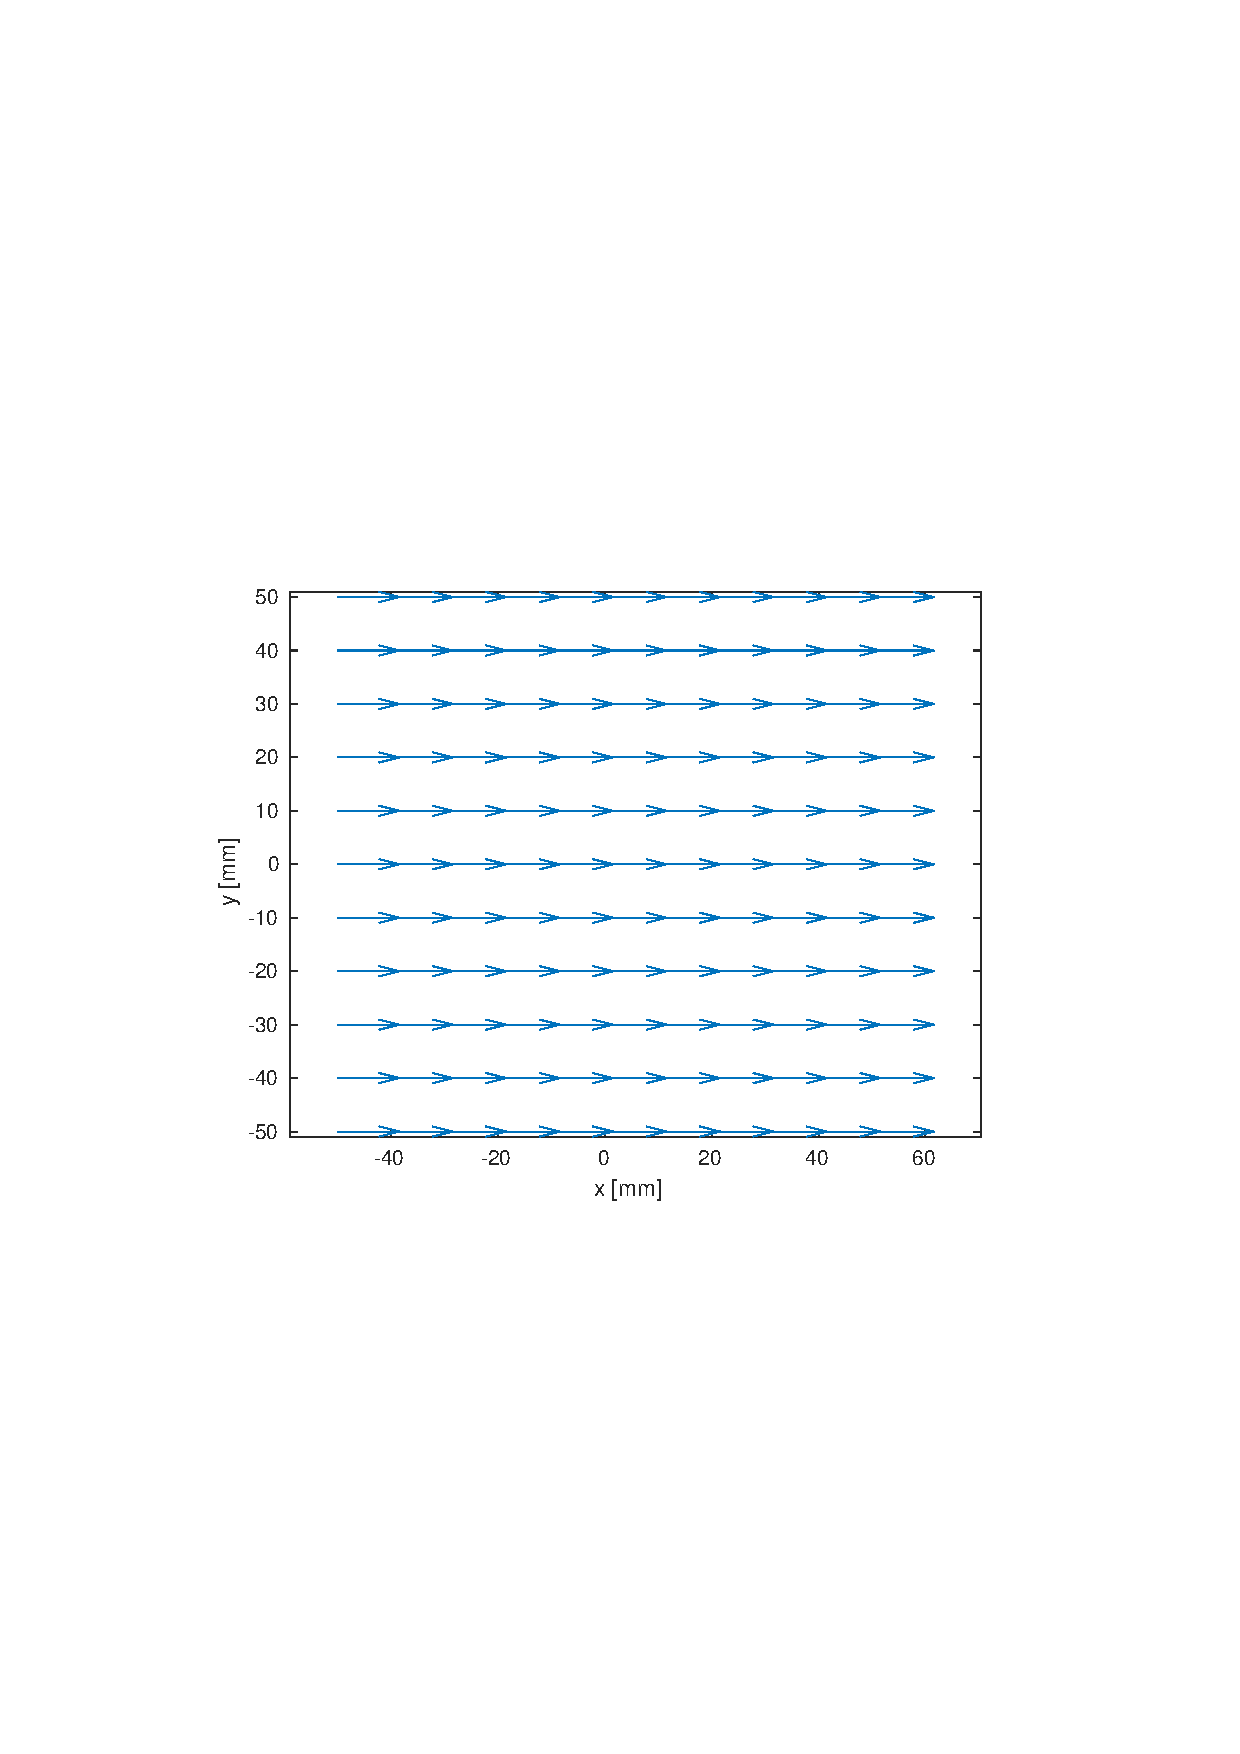
\includegraphics[clip, trim=3.5cm 8cm 3.5cm 8cm, width=0.72\linewidth]{Pictures/constant.pdf}
  \caption{A vector field showing how a constant term error ($q_{00})$  influences the measurement points.}
  \label{fig:constant}
\end{figure}

\begin{figure}[ht!]
  \centering
  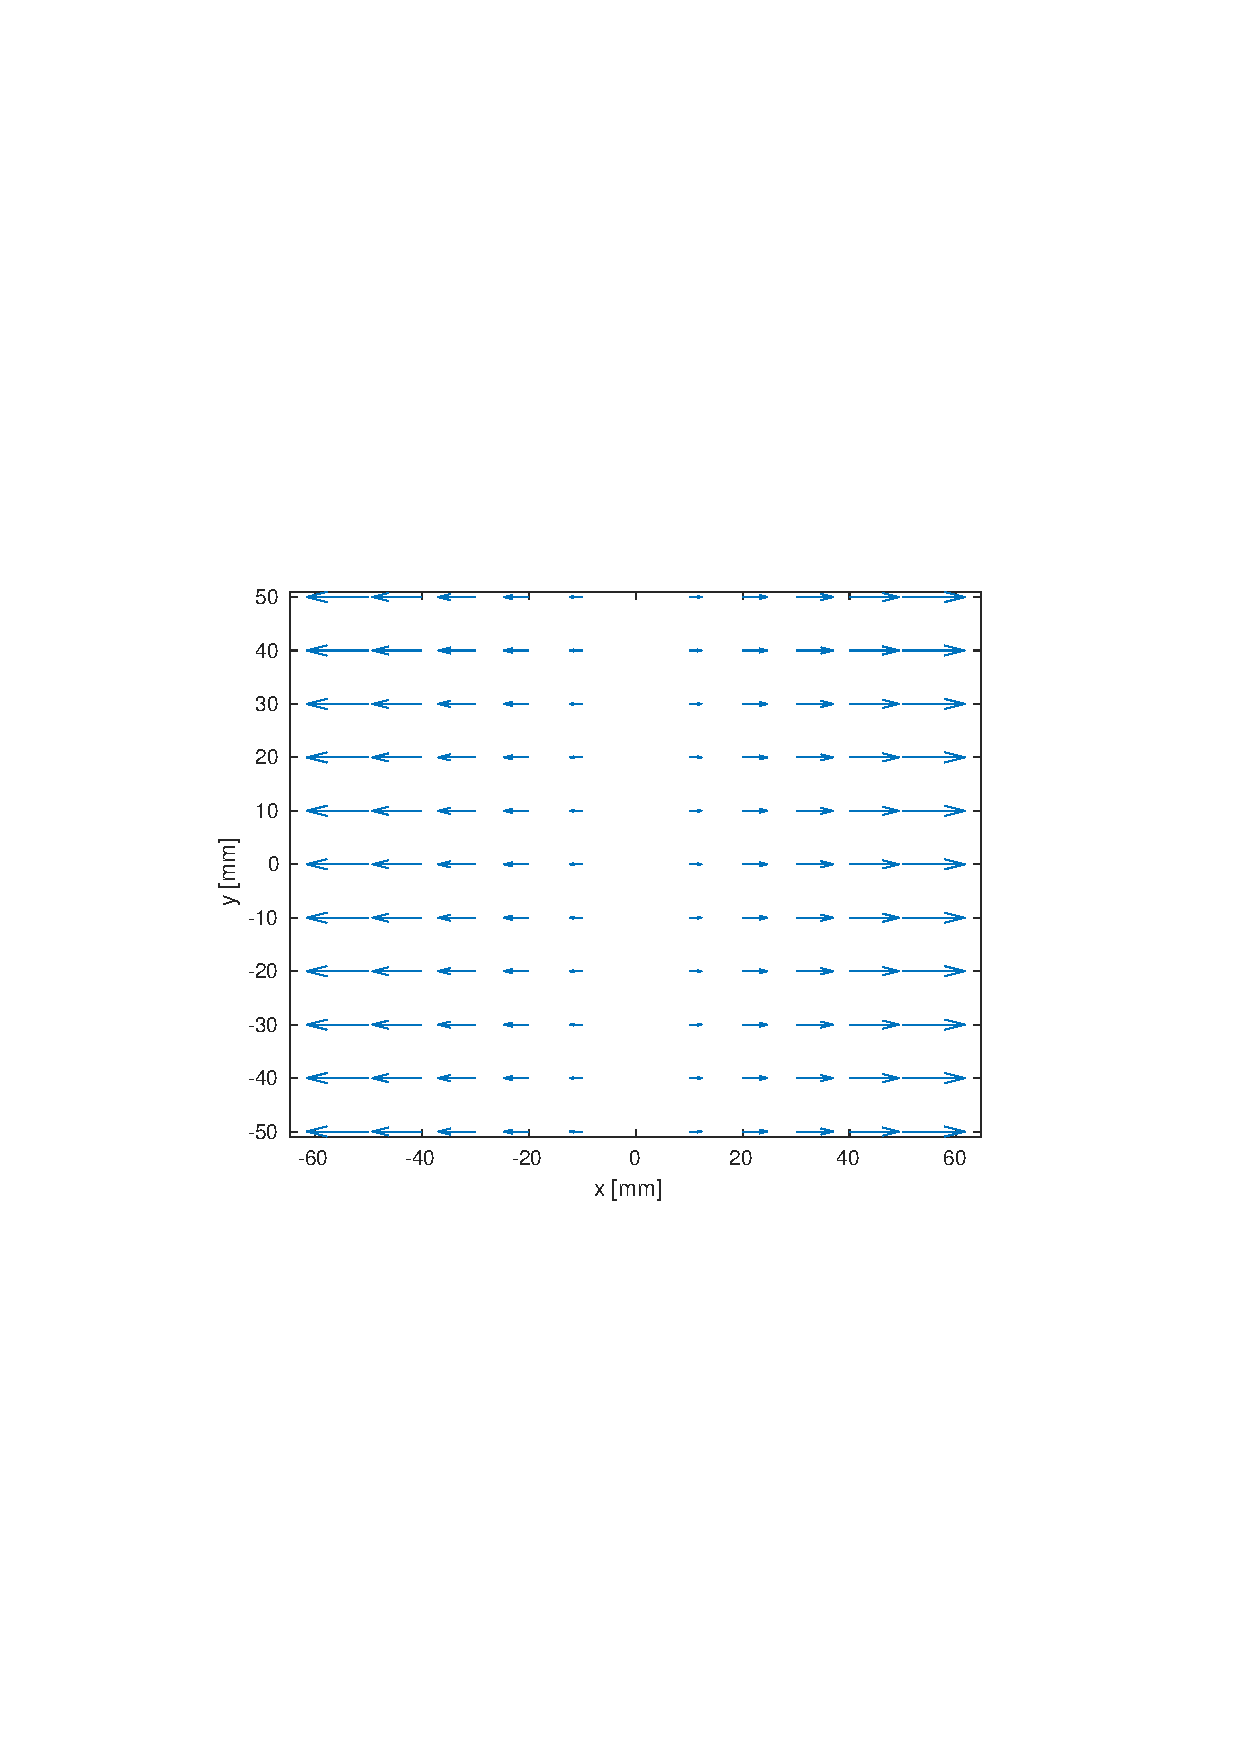
\includegraphics[clip, trim=3.5cm 8cm 3.5cm 8cm, width=0.72\linewidth]{Pictures/proportional.pdf}
  \caption{A vector field showing how a proportional term error ($q_{10})$ influences the measurement points.}
  \label{fig:proportional}
\end{figure}

Including the $q_{01}$ terms in the polynomial necessarily improves the goodness-of-fit as any extra term will. But there are also two more specific reasons to include this term. One is the consideration about rotation between build chamber and measurements, that was presented earlier. The other is the consideration about the interdependence of the x and y variables presented in Section \ref{sec:f-theta-dev-angle}. That is to say, the observation that both the nominal x and y value will have influence on both the measured x and y, which gives reason to at least include \textit{some} term containing the opposite variable in the polynomial.

When including $q_{01}$ the result is that the coefficient $q_{x01}$ turns out as 0.0014 which means $0.0014*50mm = 0.07mm$ offset in the outermost position. This is small but significant. Looking at the value of $q_{y01}$ it shows to be negative, which is in accordance with the theory that the points are rotated. But since the magnitudes of $q_{x01}$ and $q_{y01}$ are significantly different, the points are not only rotated but also sheared. The rotation can only be explained by a less-than-perfect alignment of the coordinate system during the measurements. But the shear can't be explained similarly, giving all the more reason to include the term $q_{01}$ in the model. The characteristic of the rotation/shear is depicted on Figure \ref{fig:shear}

\begin{figure}[ht]
  \centering
  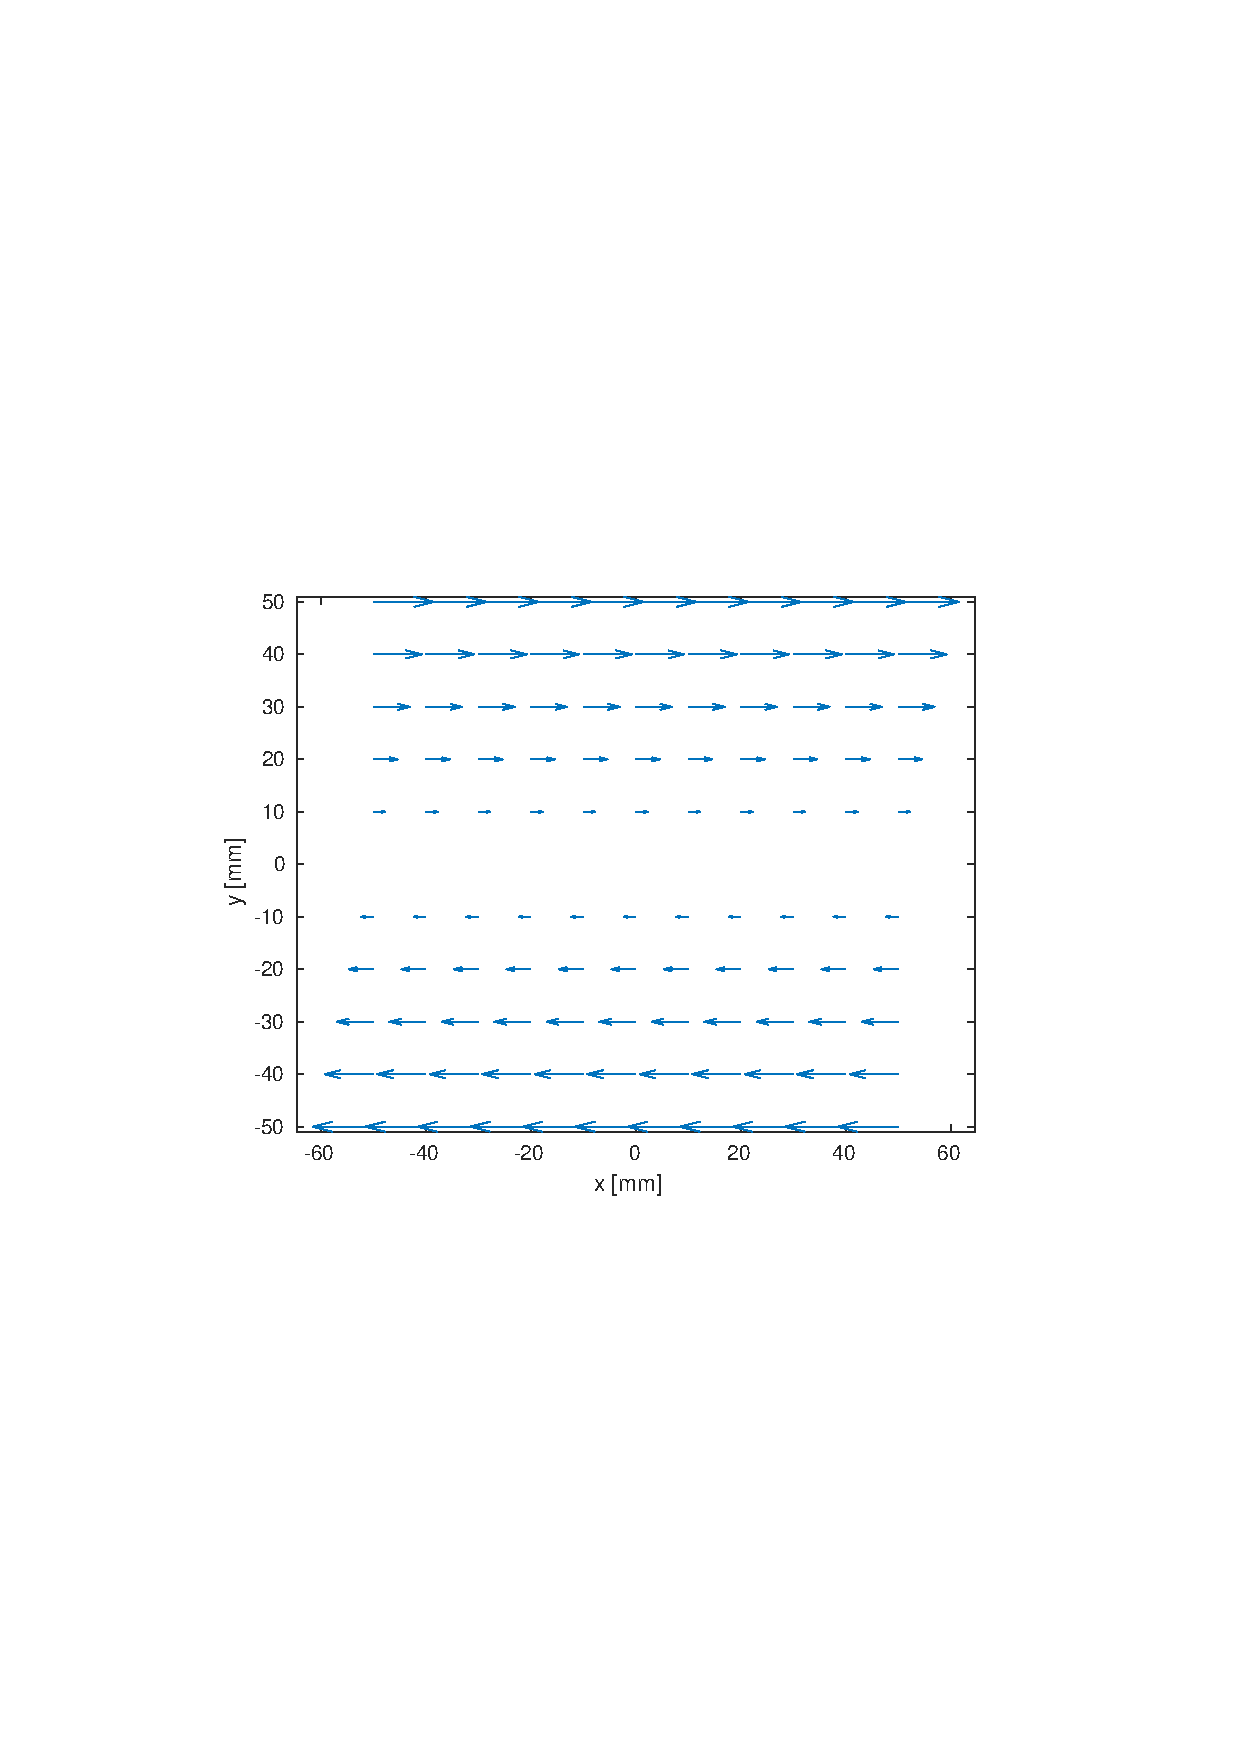
\includegraphics[clip, trim=3.5cm 8cm 3.5cm 8cm, width=0.72\linewidth]{Pictures/shear.pdf}
  \caption{A vector field showing how a rotation/shear term error ($q_{01}y)$ influences the measurement points.}
  \label{fig:shear}
\end{figure}

The third order terms with coefficients $q_{12}$ once again improve the degree of explanation a lot bringing the sum of square errors to an order of magnitude lower than the first model. This model also fits with the typical distortion characteristics of two-mirror-galvanometers, the so called "pin cushion"-effect \cite[Figure 2.35]{sebastian-phd} as shown of Figure \ref{fig:pincushion}. Unfortunately it turns out that solving for $x_{meas}$ and $y_{meas}$ with this model comes down to solving a fifth(!) order equation, which has no general solution \cite{abel-no-5}, and no specific solution for this case turned up in the literature search for this project. Implementing a correct numerical solution is beyond the scope of this report, but might very well be worth the effort. Similarly the terms $x_{nom}^3$ and $y_{nom}^3$ might be useful but are out of bounds for this project.

\begin{figure}
  \centering
  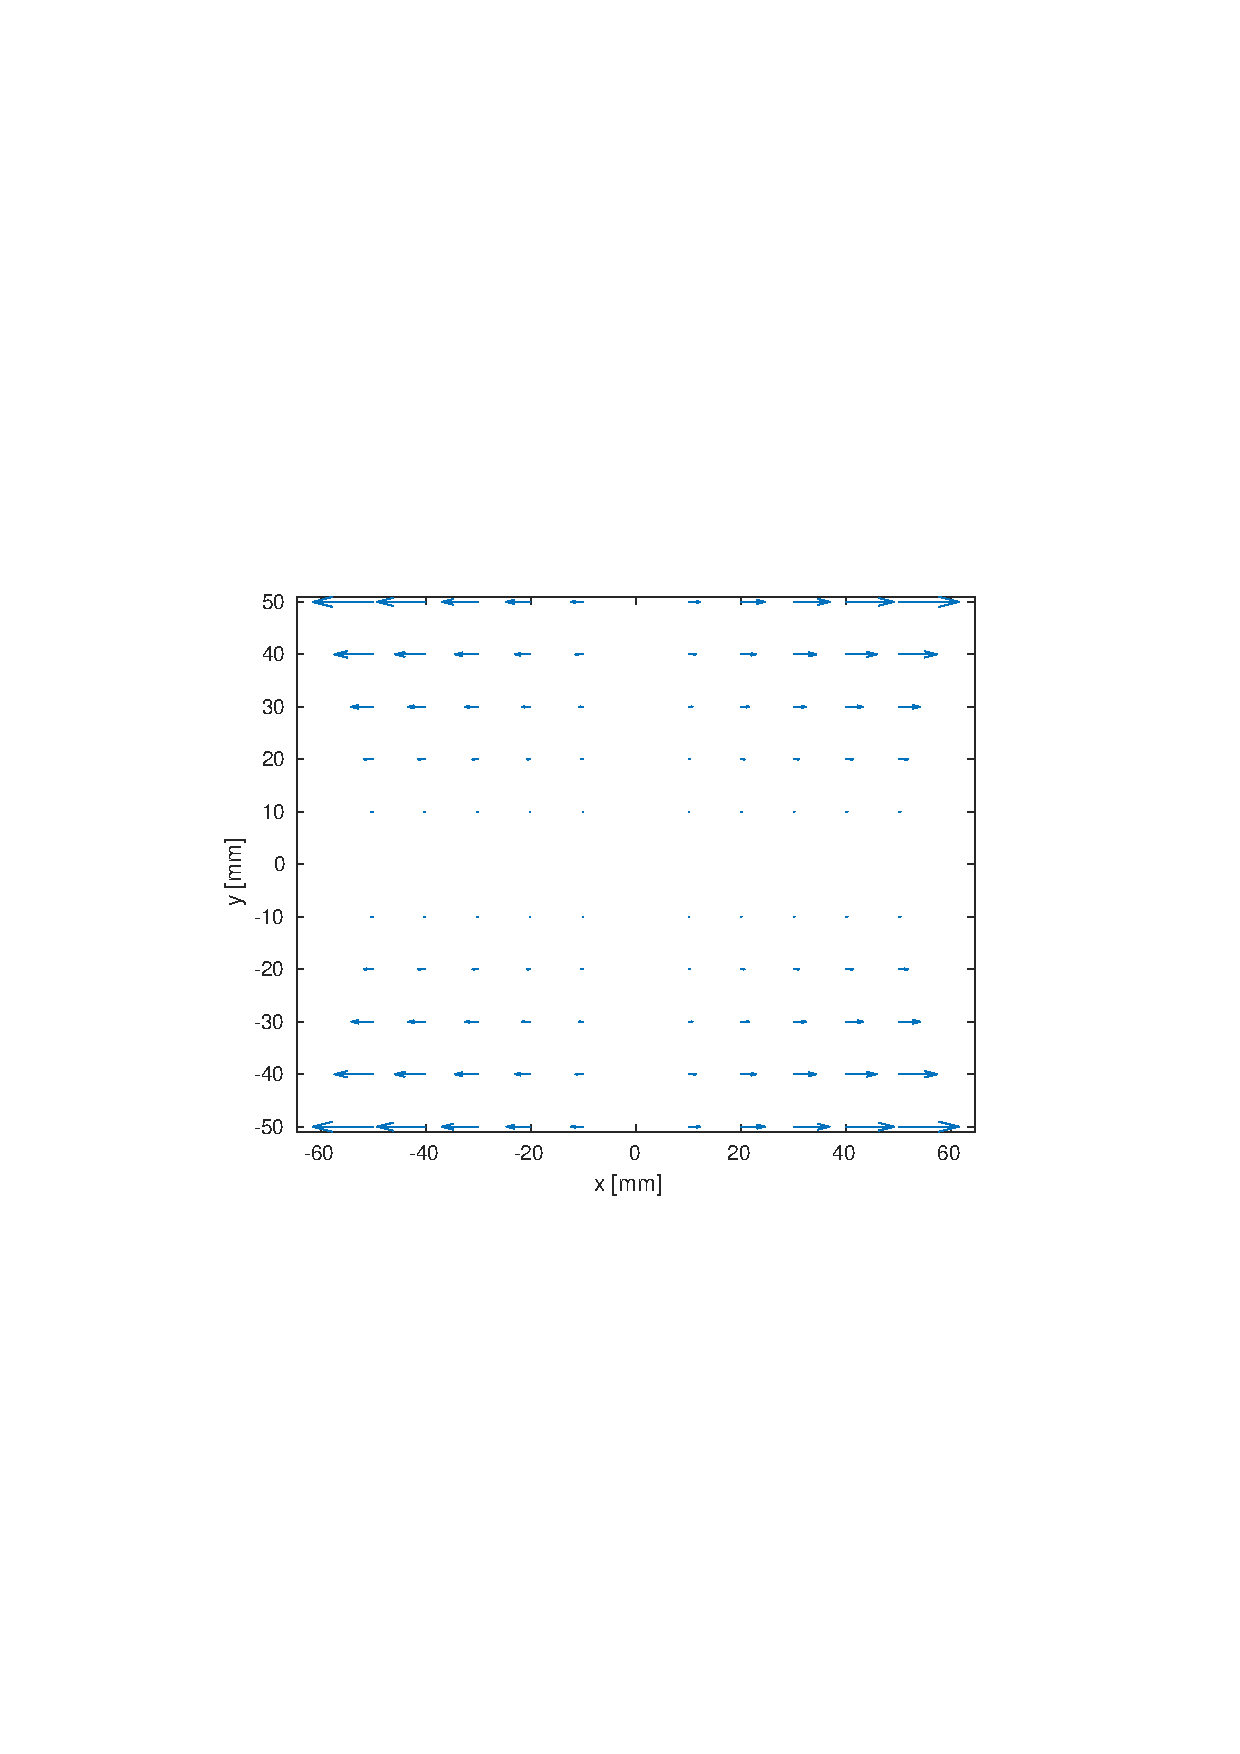
\includegraphics[clip, trim=3.5cm 8cm 3.5cm 8cm, width=0.72\linewidth]{Pictures/pincushion.pdf}
  \caption{A vector field showing how a pin cushion term error ($q_{12}y^2x)$ influences the measurement points.}
  \label{fig:pincushion}
\end{figure}

However the goodness-of-fit of the second model is satisfactory for it's purpose, so this two-variable-linear-model will be used going forward.

\subsection{Solving for nominal values}

Given the model chosen in section \ref{sec:the-fit}, the task is to solve the Equations \ref{eq:x-meas} and \ref{eq:y-meas} for the variables $x_n$ and $y_n$.

\begin{align}
x_m &= q_{x00} + q_{x10}x_n + q_{x01}y_n \label{eq:x-meas}\\
y_m &= q_{y00} + q_{y10}y_n + q_{y01}x_n \label{eq:y-meas}
\end{align}

This results in the Equations \ref{eq:x-nom} and \ref{eq:y-nom}. The results can be verified by substituting the expression for $x_n$ and $y_n$ back into the right hand side of Equations \ref{eq:x-meas} and \ref{eq:y-meas} and observe that they reduce to  $x_m$ and $y_m$ respectively.

\begin{align}
    x_{n} &= -\frac{q_{y00}q_{x01} - q_{x00}q_{y10} + q_{y10}x_m - q_{x01}y_m}{q_{x01}q_{y01} - q_{x10}q_{y10}} \label{eq:x-nom}\\
    y_n &= -\frac{q_{x00}q_{y01} - q_{y00}q_{x10} + q_{x10}y_m - q_{y01}x_m}{q_{y01}q_{x01} - q_{y10}q_{x10}} \label{eq:y-nom}
\end{align}

The right sides of these equations then are the sought for $f^{-1}$. The coefficients ($q$'s) are determined by the regression and $x_m$ and $y_m$ now become the free variables. That way one can input what the actual result is wished to be into $f^{-1}$ and find out what nominal value should to send to the printer, to actually get the original desired result. The data analysis MATLAB script is attached as Appendix \ref{app:calibration-matlab}.

\section{Implementation of calibration}

The errors that the calibration tries to adjust for come from the hardware of the printer: the mirrors, the lens, the frame. So for system design, it would be preferable to implement the corrections as close to the hardware as possible. Since it isn't an option to correct the hardware itself, this would mean implementing the correction calculations as the very last step in the GLAMS before the positions are converted to XY2-100 messages and send to the scanner.

The GLAMS however is doing its computations in real time, and there is nothing inherent to the calibration calculations that needs this. Therefore, in order to save the limited resources of the GLAMS, the calculation are instead moved to just before the g-code sender. This also works, because nothing influences the calibrated positions in or after the g-code sender.

More specifically the calculations are implemented as a python script (see Appendix \ref{app:calibration-g-code-python}) that finds the coordinates in the g-code script and converts them from naive to calibrated, with the function $f^{-1}$ above. The placement of the python script in the system diagram is shown on Figure \ref{fig:system-overview-w-cal}

\begin{figure}[H]
    \centering
    \includesvg[width=0.45\linewidth]{Pictures/system-overview-w-calibration.svg}
    \caption{The upper right corner of the system diagram in Figure \ref{fig:system-overview} but with the calibration script added}
    \label{fig:system-overview-w-cal}
\end{figure}

\section{Verification of calibration}

To verify if the calibration had helped, an identical production process as the one described in the calibration medium production (Section \ref{sec:cal-medium-prod}) was done. This time however, the g-code was first adjusted with the calibration script, so that all the coordinates were calibrated. Then it was measured with the same procedure as in Section \ref{sec:cal-meas} and the same data analysis was performed as in Section \ref{sec:cal-cal}. The measurement results are attached as Appendix \ref{app:verification-data}. For this second data analysis, the main metric of interest was how close the $q_{10}$ terms were to 1.

\subsection{Calibration results}

The results of the data analysis are shown in Table \ref{tab:cal-ver-fits}. For the x-position a drastic improvement has been achieved, even with the 95\%-confidence interval crossing over 1. For the y-position a small but significant improvement has been achieved (The uncalibrated result of 0.9933 is outside the confidence interval). It should also be noted that the $q_{01}$ variables now are of similar magnitude with opposite sign, meaning there no longer is any sign of shear, only rotation. It must be concluded that the calibration procedure as laid out in this chapter has been a success.

\begin{table}[ht]
    \centering
    \begin{tabular}{l|c|c}
        $q$ & 
        $x_m = q_{x00} + q_{x10}x_n + q_{x01}y_n$ & $y_m = q_{y00} + q_{y10}y_n + q_{x01}x_n$ \\
        \hline
        $q_{00}$ & -0.0406 [-0.0483, -0.0330] & -0.0035 [-0.0144, 0.0074]  \\
        $q_{10}$ & 0.9999 [0.9997, 1.0002] & 0.9952 [0.9946, 0.9956] \\
        $q_{01}$ & -0.0004 [-0.0006, -0.0002] & 0.0003 [-0.0001, 0.0006] \\
        SSE & 0.0014 & 0.2865
    \end{tabular}
    \caption{Coefficients with 95\%-confidence intervals in brackets found by regression of control data (see Appendix \ref{app:verification-data}) to the expressions in the top}
    \label{tab:cal-ver-fits}
\end{table}

The calibration showed to be a good way to get a more accurate position of the laser, but position is not the only aspect of the scanner movement that is of interest. The velocity is very important as well and is determined by the trajectories of the scanner, that is, the changes of position over time.


